\documentclass[]{article}
\usepackage[UTF8]{ctex}
\usepackage{graphicx}
\usepackage{amsmath}
\newtheorem{definition}{Definition}
\newtheorem{theorem}{Theorem}

%opening
\title{对称加密的一种具体安全处理\footnote{原文:M. Bellare, A. Desai, E. Jokipii and P. Rogaway, "A concrete security treatment of symmetric encryption," Proceedings 38th Annual Symposium on Foundations of Computer Science, 1997, pp. 394-403, doi: 10.1109/SFCS.1997.646128.}}
\author{作者:M. Bellare,A. Desai,E. Jokipii,P. Rogaway\\
\small{译者:李晓峰,北京联合大学智慧城市学院\footnote{译者email:cy\_lxf@163.com,译文来自于译者发起的“信息安全经典翻译”开源项目https://gitee.com/uisu/InfSecClaT}}
}

\begin{document}

\maketitle

\begin{abstract}
我们在具体安全(concrete security)框架内研究对称(如私钥)加密方案的概念。\par
我们给出四种不同的抵抗选择明文攻击(chosen plaintext attack)的安全概念,分析这些概念之间规约的具体复杂度,提出了上下限,并获得了这些概念间的紧密关系。利用这样的方法,我们对概念根据在具体安全方面更强或更弱进行了分类(尽管相互间可以多项式规约)。\par
接下来我们提供了分组密码加密方法的具体安全性分析,包括最流行的加密方法CBC,我们将对手模型化为他们的资源函数,从而建立了严格的界限(意味着匹配上界和攻击)。
\end{abstract}

\section{引言}
加密方案使Alice能够以这样的方式向Bob发送消息,即敌方Eve不会获得关于消息内容的重要信息。这是密码学的经典问题。通常在两种设置中考虑。在对称(私钥)系统中,加密和解密是在发送方和接收方共享的密钥下执行的。在非对称(公钥)设置中,发送方具有一些公共信息,接收方持有一些相应的秘密信息。\par

在本文中,我们有两个目标。第一个是在具体安全框架中研究对称加密的概念。这意味着我们将研究不同概念之间的规约的具体复杂性。我们想证明上下界。通过这种方式,我们可以在概念之间建立紧密的关系,并可以比较概念(即使彼此可多项式规约)的强弱。\par

第二个目标是提供一些特定对称加密方案的具体安全性分析。我们考虑的其中一种方案(CBC加密)是普遍使用的,但在传统可证明安全性中从未进行形式化分析(具体或其他)。我们想纠正这一点。同样,目标是找到对手成功概率的严格界限,作为其消耗资源的函数。这包括证明上界和匹配下界。

\subsection{背景和动机}
Goldwasser和Micali的开创性工作[11]是第一个为加密引入安全的形式化概念。具体来说,他们提出了非对称加密的两个安全概念,“语义安全”和“多项式安全”,并证明了它们在多项式时间规约方面是等价的。Micali、Rackoff和Sloan[17]表明,这些概念的(适当版本)也等同于姚[20]提出的另一个概念。Goldreich[8]给出了非对称加密概念的统一复杂性处理。Luby[15,第11-12章]提出了这些概念对对称设置的一些修改。
\par

Goldwasser和Micali[11]还提出了一种非对称加密方案,其安全性(在上述意义上)是可从二次剩余多项式时间规约。随后,基于各种难题,出现了许多其他方案。\par

\textbf{{\large 具体安全(concrete security).}}
上述所有工作的观点是,如果两个安全概念之间存在多项式时间规约,则它们是等价的;并且如果从一个困难问题到一个方案存在多项式时间规约,则该方案被声明为可证明安全的。这些当然是基本问题,但我们认为,一旦知道答案,就必须以更精确的方式对概念和方案进行分类。\par

打个比方,只关心密码学中的多项式时间可约性有点像只关心计算问题是否在P中。然而,我们知道有许多有趣的问题(包括算法领域的大部分,以及复杂性理论)围绕着获取关于已知在P中的问题的进一步信息。这些信息有助于更好地理解问题,对于实际应用也是必不可少的。\footnote{译者注:打比方是为了用一个大家都知道的东西做类比,编译理解新的问题或较难的问题,Bellare是学数学出身,估计他认为大家应该对计算复杂性都有了解,所以用这个打比方。}
\par

在密码学中注意多项式等价概念的具体复杂性具有类似的结果。特别是,当规约不是保持安全(security-preserving)时,这意味着必须使用更大的安全参数才能安全,从而降低效率。因此,最终,我们为低效规约在保证或运行时间方面付出了代价。\par

我们的具体安全方法是[5,6]的方法,其中一种方法参数化了所涉及的资源,并通过其上\footnote{译者注:这里的“其上”是指参数化的资源。}的显式函数来衡量对抗成功。该方法是非渐近的,适用于具有有限域的函数。\par

我们将不仅关注通过展示具体边界来证明安全性,还关注通过展示匹配攻击来证明这些边界是最好的。同样,我们遵循[3,5]这样的工作,他们为某些消息身份验证方案做了这样的工作。\par

尽管本文关注的是对称加密的具体安全性,但我们认为,总体而言,具体安全性是理论密码学中一种新兴的富有成效的研究途径。

\subsection{安全概念}
我们将考虑对称加密的四个安全概念,并检查它们之间的规约复杂性。第一个概念,我们称之为“真实或随机不可区分性(real-or-random indistinguishability)”,是新概念,第二个概念,“左或右不可区分(left-or-right indistinguishability)”是其变体。接下来的两个概念,“查找-猜测安全(find-then-guess security)”和“语义安全(semantic security)”是[11]的概念对对称加密的变种。我们的目标是在所有概念中模型化选择明文攻击。\par

如上所述,我们的具体安全方法是通过参数化对手A的资源。我们区分A的运行时间t(根据惯例,我们在其中包括A程序的空间);A看到的密文数量$\mu$;A向加密oracle进行的查询数量q。(要模型化选择明文攻击,我们必须让对手能够看到密码。在公钥方案中,她可以在给定公钥的情况下自己创建密码文本,但在对称加密方案中,加密密钥是保密的,因此我们必须修改模型,并为对手提供具有加密功能的oracle。加密oracle的存在是“将对称加密的概念视为非对称加密的特例”不正确的一个原因。)
着眼于实际应用,将所有这些资源分开处理是很重要的。(以前的工作忽略了q和$\mu$,因为它们受t的限制。但作为资源,它们非常不同,因为通常,获得合法密文比执行局部计算更困难。)因此我们得到了$(t,q,\mu;\epsilon)$安全($(t,q,\mu;\epsilon)-security$)的概念,这意味着当对手拥有支出的这些资源时,其成功概率最多为$\epsilon$。当然,衡量成功概率的方法在四个不同的概念中有所不同。\par

\subsection{概念间的规约}
我们证明了“真实或随机不可区分性”和“左或右不可区分”是等价的,规约至一个小的常数因子。(也就是说,我们在它们之间有安全性保持规约。)我们还展示了从这些概念到"查找-猜测安全"的拿权保持性规约。然而,从"查找-猜测安全"到“左或右不可区分”(或“真实或随机不可区分性”)并不是安全性保持的。然而,我们表明,我们给出的规约是严格的,我们不能指望有更好的结论。\par

我们展示了一种从语义安全到"查找-猜测安全"的安全性保持规约。在另一个方向上,我们规约的复杂性取决于“信息函数”f(表示明文语义安全的属性)的时间复杂性和“消息空间采样算法(message-space sampling algorithm)”。如果这些复杂性较低,则规约是好的。\par

从以上结果可以清楚地看出,当人们想要证明某种加密方案$\Pi$的安全性时,最好是从“真实或随机不可区分性”或“左或右不可区分”给出一个严格的规约,因为这意味着对其余部分\footnote{译者注:“其余部分”是指其余的安全概念}也会有好的规约存在,图\ref{Fig:fig1}给出了规约的总结。\par

\begin{figure}[htbp]
	\centering
	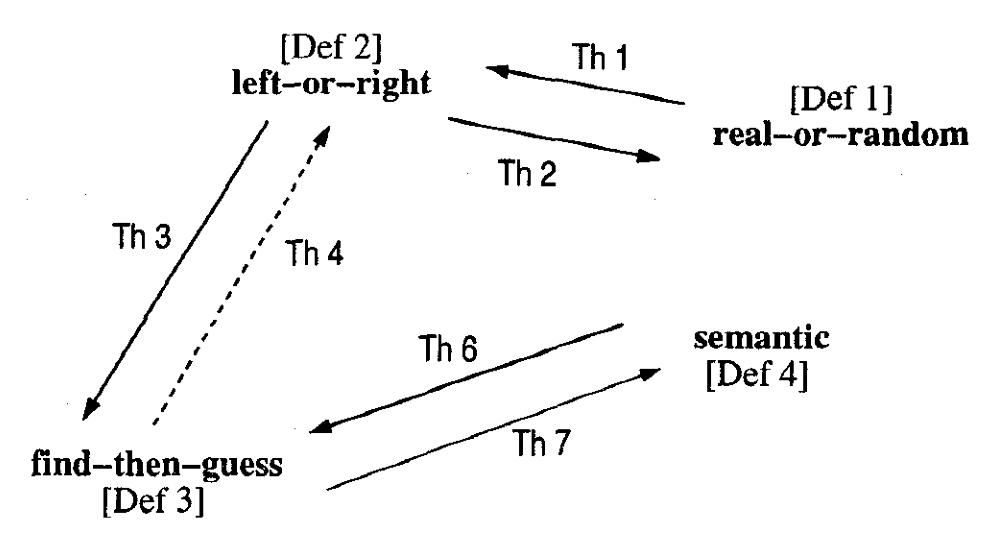
\includegraphics[width=0.8\textwidth]{Fig1.png}
	\caption{概念间的关系,从概念A到概念B的实线表示存在从A到B的安全性保持规约,A到B的虚线表示规约是安全性不保持的。}
	\label{Fig:fig1}
\end{figure}

虽然之前在方案分析的背景下考虑过具体安全性,但这是这是第一次考虑不同安全性概念之间关系的工作。也就是说,这是第一次根据概念之间规约的复杂性将概念划分为较弱或较强。\par

实际上,这些结果很容易扩展到非对称方案。我们主要关注对称方案,因为这是我们要分析的方案所在的领域。

\subsection{加密方案的安全性}

我们分析了一些经典对称加密方案的安全性。具体来说,我们研究了使用分组密码(例如DES)的两种不同加密模式:CBC(密码块链接模式);和XOR(有时称为计数器模式)。对于后者,我们同时考虑概率和状态两种情况。\par

在这些方案中,底层本原(underlying primitive)\footnote{primitive有翻译为“原语”的,这里采用“本原”的翻译,保持了于冯登国老师在以下这篇文章中的翻译一致:冯登国. 可证明安全性理论与方法研究[J]. 软件学报, 2005, 16(10):14.}是伪随机函数(PRF)或伪随机置换(PRP)族F,
其中由密钥a指定的特定函数$F_a$将l比特映射到L比特,其中l和L是固定的
(对于置换,I=L)。为了加密消息,$F_a$的应用以某种依赖于方案的方式迭代( iterated)。我们希望看到加密方案的安全性如何取决于PRF族的假定安全性。我们定义了PRF和PRP族的具体安全性,如[6]中所述,通过时间t’、oracle查询数量q’和区分器(distinguisher)的最大优势$\epsilon '$的参数化。那么问题是:假设F是($(t',q';\epsilon ')$安全($(t',q';\epsilon ')-security$)的PRF族,那么$t,q,\mu ,\epsilon$的值是什么,使得加密方案是$(t,q,\mu;\epsilon)$安全的?我们寻求上界和下界。(后者代表了最著名的攻击。)
\par

对于有状态XOR方案,我们证明了该方案对于$\epsilon =2 \epsilon ',\mu =q'l$和t与t’仅相差一个加法量 是 $(t,q,\mu;\epsilon)$安全的,这意味着该方案与我们可能希望得到的方案一样好。对于概率XOR方案,我们证明了该方案对于$\epsilon =2 \epsilon '+\mu (q-1)/(L2^l),\mu =q'l$
和t与前面描述一致的情况下是$(t,q,\mu;\epsilon)$安全。对于CBC,参数值是$\epsilon=2\epsilon '+(\mu^2 - \mu l)/(l^22^l),\mu=q' l$。在所有情况下,我们证明这些结果是严格的(tight),直到一个常数。我们得出结论,基于有限PRF的有状态XOR具有最佳安全性。
\par

上面所说的安全性是在“左或右不可区分”意义上的。根据我们之前所说的,这给出了其他三个概念一个可以比较的边界。

\subsection{更多历史}

我们已经提到了最重要的相关工作,即[11]。这里我们提供了一些更详细的比较和历史,并讨论了其他工作。\par

我们的结果表明,我们所考虑的概念在多项式时间规约下是等价的,因此可以在一个层面上将其视为对称情况下的[11]的模拟(analogue)。\par

在讨论不对称方案时,文章[8]表示对称方案可以类似地处理。这种观点中缺少的一个要素是,为了模型化选择明文攻击,必须在对称方案中为敌手提供某种加密手段。我们通过向对手提供加密预言(encryption oracle)来扩展多项式和语义安全。\par

也出现了比[11,17]更强的非对称加密概念,包括[19,7],但我们的关注仅限于在选择的明文攻击下保护隐私。\par

Luby[15]定义了对称加密的“发现-猜测安全”本质上是什么,他提到了使用伪随机函数族的加密,其输出长度是您希望加密内容的比特位数。他的处理方法对规约效率给予了一定的关注(尽管他并不像我们一样关注具体安全性)。\par

奇怪的是,一些早期的工作有一个更具体的处理方法:在非对称加密领域,Alexi等人[1]仔细地表明了其规约的复杂度,但后来许多工作不幸放弃了这一习惯。\par

从单向函数构造伪随机发生器[13]为从单向函数开始的对称加密提供了解决方案。在目前的工作中,存在不是问题\footnote{译者注:这句话的意思应该是“前面那种方案的存在不是问题”。};我们感兴趣的是具体安全性和对某些特定方案的分析。\par

[6]中提供了CBC MAC的具体安全性分析。(CBC MAC不应与CBC加密混淆:前者是消息身份验证代码。)我们基于他们的技术,但这些技术并不能直接解决这里的问题。CBC模式加密在[2,14,18]中标准化。

\subsection{关于此摘要文章}
本文一个扩展摘要,仅包含定义、方案描述和结果陈述。由于篇幅限制,证明被省略。我们论文的完整版本,包括所有证明,可以在[4]中找到。

\section{加密的概念}
对于所有复杂度度量,修复一些概率RAM模型(For all complexity measures fix some probabilistic RAM
model.)。我们采用的约定是“时间”是指实际运行时间加上代码大小(相对于某些固定编程语言)。Oracle查询以单位时间回答。\par

如果$A(.,.,...)$是任何概率算法,则$a\leftarrow A(x_1,x_2,...)$表示在输入$x_1,x_2$上运行A的实验,并将$a$作为输出,概率是A的投币概率(the probability being over the coins of A.)。类似地,如果A是集合,则$a\leftarrow A$表示从A中均匀选择点并分配该值的实验。

\subsection{加密方案的语法}
将这些硬币(Coins)记为${0,1}^\infty$(无限字符串的集合),设$MsgSp\subseteq {0,1}*$是集合,消息空间,其中$x\in MsgSp$ 意味着每个与$x$具有相同长度的字符串$x'$,有$x'\in MsgSp$, 设$KeySp\subseteq {0,1}*$是集合,表示密钥空间, 设$CipherSp={0,l}*$。
\par

 \textbf{\large{无状态加密(STATELESS ENCRYPTION).}} 一个(概率,无状态,对称)加密方案是一个三元组$\Pi=(\varepsilon,D,K)$:\par
 
$\varepsilon : KeySp\times MsgSp \times Coins\rightarrow CipherSp$\par
$D : KeySp\times CipherSp \rightarrow MsgSp$\par
$K :  Coins\rightarrow KeySp$\par

算法$\varepsilon$称为加密算法;$D$是解密算法;$K$是密钥生成器:我们要求对于所有$a\in KeySp$,$x\in MsgSp$,$r\in Coins$和$D(a,\varepsilon(a,x,r))=x$。我们通常将第一个参数即密钥作为下标写入$\varepsilon$和$D$。我们称$\varepsilon_a(x,r)$为密钥$a$和硬币$r$下明文$x$的加密,或者更简洁地称为密文。我们将$D_a(y)$称为密钥$a$下密文$y$的解密。通常我们忽略了自变量$K$,将$K$视为概率算法,或是诱导概率空间(induced probability space)。类似地,我们经常忽略$\varepsilon$的最终参数,将$\varepsilon_a$视为概率算法,或将$\varepsilon_a(x)$视为诱导概率空间。在$y$不是密钥$a$下的任何字符串$x$的密文的情况下,记为$D_a(y)=\perp$。
\par

对于一个有用的加密方案,$\varepsilon,D,K$应该是可有效计算的函数,但安全性的概念在这方面没有正式要求(formal demands,也可译为“形式化要求”)。\par

 \textbf{\large{有状态加密(STATEFUL ENCRYPTION).}}
 我们还考虑有状态加密方案,其中密文是一些信息的函数,如计数器,由加密方维护,并随每次加密而更新。在形式上,这种方案与之前的方案具有相同的语法,除了
 \[\varepsilon:KeySp \times MsgSp \times St \times Coins\rightarrow St \times CipherSp,\]
此处$St\subseteq \{0,1\}*$是一组可能的状态,包含一个可区分的状态,空字符串$\epsilon$,我们称之为初始状态。设$\varepsilon^i(i=1,2)$表示$\varepsilon$的第i个分量。密文现在是(输出)$\varepsilon^2$,而$\varepsilon^1$是更新状态,由发送方存储,并用作加密函数下一次应用的第三个参数。请注意,加密变为有状态,但解密不会。
\par

\subsection{四个安全概念}
我们现在给出了四个安全概念,每个概念都模拟了选择明文攻击。在每种情况下,我们都允许对手以某种形式访问加密oracle;这是这些定义区别于以前定义的一个特征。我们将描述无状态加密方案的定义,并在后面说明如何为有状态加密方案修改它们。
\footnote{译者注:原文以下内容并无标号,只是字体加粗大写,此处为了便于阅读将其排版为三级带标号标题。}
\par

\subsubsection{真实或随机(REAL-OR-RANDOM)}

其思想是,敌手无法区分文本加密和等长垃圾字符串加密。(通过传递性,敌手无法区分任何两个等长字符串的加密。)形式化考虑了两个不同的游戏。在游戏1中,我们首先选择一个随机密钥$a\leftarrow K$。然后给敌手一个Oracle,当向此Oracle询问字符串$x\in MsgSp$时,该Oracle用密钥a下的x(随机)加密进行响应。在游戏2中,我们开始选择随机密钥$a\in K$,然后,给对手一个Oracle,当向此Oracle询问字符串$x\in MsgSp$时,Oracle用它用长度为$|x|$的随机字符串的(随机)加密(在密钥a下)进行响应。如果没有“公平(reasonable)”敌手在区分游戏1和游戏2中获得“显著”优势,则加密方案是“好的”。\par

\begin{definition}[真实或随机(REAL-OR-RANDOM)]
	我们说加密方案$\Pi =(\varepsilon,D,K)$在“真实或随机”意义( real-or-random sense)上是$(t,q,\mu;\epsilon)$安全,当以下条件成立:
	\[Adv_A^{rr} \stackrel{def}{=} Pr[a\leftarrow K:A^{\varepsilon_a(\cdot)}=1] - Pr[a\leftarrow K : A^{\varepsilon_a(\$|\cdot|)}=1]\]
	$Adv_A^{rr} \leq \epsilon$,对于任意敌手A,其运行的时间最多为t,询问Oracle最多q次,这些总计最多为$\mu$比特。
\end{definition}

$A^{\varepsilon_a(\cdot)}$表示$A$有一个Oracle,A向此Oracle查询$x$,Oracle返回$y\leftarrow \varepsilon_a(x)$.(这意味着它选择一个随机字符串$r$并返回$\varepsilon_a (x,r)$,每次调用Oracle时都会选择一个新的随机字符串。)$A^{\varepsilon_a(\$|\cdot|)}$表示$A$有一个Oracle,A向此Oracle查询$x$,Oracle先选择$x'\leftarrow \{0,1\}^{|x|}$,然后返回$y\leftarrow \varepsilon_a(x')$做为响应.
\footnote{译者注:此定义表明两种不同Oracle都返回1的概率之差小于$\epsilon$。}

\subsubsection{左或右(LEFT-OR-RIGHT)}
我们再次考虑两个不同的游戏。在这两种游戏中,查询都是来自MsgSp的等长字符串对$(x_1,x_2)$。在任一游戏中,我们首先选择一个随机密钥$a\leftarrow K$,并在游戏期间固定该键,在游戏1中,一个oracle接收$(x_1,x_2)$用来自$\varepsilon_a(x_1)$的随机样本进行响应。在游戏2中,它使用来自$\varepsilon_a(x_2)$的随机样本进行响应。因此,游戏1提供了“左”Oracle,而游戏2提供了“右”Oracle。如果“公平”敌手无法在区分游戏1和游戏2时获得“显著”优势,我们认为加密方案是“好的”。

\begin{definition}[左或右(Left-or-Right)]
	我们说加密方案$\Pi =(\varepsilon,D,K)$在“左或右”意义( Left-or-Right sense)上是$(t,q,\mu;\epsilon)$安全,如果对于任意敌手$A$,其运行的时间最多为t,询问Oracle最多q次,这些总计最多为$\mu$比特,且:
	\[Adv_A^{lr} \stackrel{def}{=} Pr[a\leftarrow K:A^{\varepsilon_a(left(\cdot,\cdot))}=1] - Pr[a\leftarrow K : A^{\varepsilon_a(right(\cdot,\cdot))}=1]\]
	$Adv_A^{lr} \leq \epsilon$。
\end{definition}
$A^{\varepsilon_a(left(\cdot,\cdot))}$表示$A$有一个Oracle,返回$y\leftarrow \varepsilon_a(x_1)$做为查询$(x_1,x_2)$的响应。
$A^{\varepsilon_a(right(\cdot,\cdot))}$表示$A$有一个Oracle,返回$y\leftarrow \varepsilon_a(x_x)$做为查询$(x_1,x_2)$的响应。

\subsubsection{查找-猜测(FIND-THEN-GUESS)}
这是对[ll,17]中给出的多项式安全概念的调整,我们想象一个分两个阶段运行的对手A,在敌手的“查找阶段(find stage)”,她努力想出一对长度相等的消息$x_0,x_1$,她想尝试区分它们对应的密码。她还保留了一些状态信息s,以便以后可能帮助她。在敌手的“猜测阶段(guess stage)”,她获得了一个明文$x_0$或$x_1$的随机密文$y$\footnote{译者注:这里随机的意思是“$x_0$和$x_1$之间随机取一个加密”},以及状态信息s。如果敌手正确识别了哪个明文与y对应,则敌手“获胜”。如果“公平”的对手在一半以上的时间内不能明显获胜,则加密方案是“好的”。
\begin{definition}[查找-猜测(Find-then-Guess)]
	我们说加密方案$\Pi =(\varepsilon,D,K)$在“查找-猜测”意义上是$(t,q,\mu;\epsilon)$安全,如果:
	\[Adv_A^{lr} \stackrel{def}{=} 2\cdot Pr[a\leftarrow K;
	(x_0,x_1,s)\leftarrow A^{\varepsilon_a(\cdot)}(find);
	b\leftarrow\{0,1\};
	y\leftarrow \varepsilon_a(x_b):A^{\varepsilon_a(\cdot)}(guess,y,s)=b
	]-1\]
	对于任意敌手$A$,$Adv_A^{lr} \leq \epsilon$,其运行的时间最多为t,询问Oracle最多q次,这些总计最多为$\mu$比特。
\end{definition}

据了解,上述要求$|x_0|=|x_1|$,乘2和减1只是比例因子,使得数值0对应于无优势,数值1对应于完全优势(perfect advantage)。\par

\subsubsection{语义(SEMANTIC)}
Goldwasser和Micali[11]解释了语义安全,他们说,在给定密文的情况下,可以有效计算明文的任何内容也可以在没有密文的条件下计算。我们采用[11,17]对于对称方案的形式化,设$f:MsgSp\rightarrow \{0,1\}^*$是明文$x$的某个函数,该函数表示x的信息,x是敌手试图找出的(The function represents the information about x that the adversary is trying to figure out.)。赋予MsgSp概率分布,
更具体地说,对于任何整数m,消息空间上的m分布(m-distribution)是MsgSp上概率分布的集合$M=\{M_\gamma\}_{\gamma\in \{0,1\}^{\leq m}}$,由字符串$\gamma\in \{0,1\}^{\leq m}$索引。
我们假设每个分布都是有效的,这意味着对于所有$\gamma$,$M_\gamma$中所有非零概率的字符串都具有相同的长度,并且该长度最多为$m$。设$p_{f,M_\gamma}^* = max_{y^*}\{Pr[x\leftarrow M_\gamma : f(x)=y^*]\}$,这是最可能的$f(\cdot)$值的概率。


我们的敌手将分为两个阶段。在敌手的选择阶段,它努力提出有利的分布$M_\gamma$。在对手的预测阶段,根据分布$M_\gamma$选择的明文x给出随机密文y,并希望猜测$f(x)$。如果没有公平敌手A能够以显著优于$p^*_{f,M_\gamma}$的概率猜测$f(x)$,则加密方案对于函数$f$和分布$M$是语义安全的。


先前的形式化要求所有函数f此条件成立,在我们的具体处理中,函数$f$和概率分布$M$都成为参数,因此我们可以测量明文的特定属性在特定分布下受到保护的程度。


\begin{definition}[语义(Semantic)]
	设$f: MsgSp \rightarrow \{0,1\}^*$是一个函数,$M=\{M_\gamma\}_{\gamma\in \{0,1\}^{\leq m}}$是一个在MsgSp上的m-分布,加密方案$\Pi =(\varepsilon,D,K)$在“语义”意义上是$(t,q,\mu;\epsilon)$安全,对于$M$上的$f$,如果\par
	\begin{align*}
		Adv^{sm}_A(f,M) \stackrel{def}{=} & E[a\leftarrow K;(\gamma,s)\leftarrow A^{\varepsilon_a(\cdot)}(select):\\
		 & \alpha (a,\gamma,s)]\leq \epsilon,	 where\\
		 \alpha (a,\gamma,s)=& Pr[x\leftarrow M_\gamma;y\leftarrow \varepsilon_a(x): \\
		                     & A^{\varepsilon_a(\cdot)}(predict,y,s)=f(x)]-p^*_{f,M_\gamma},
	\end{align*}
	对于任何敌手A,其运行的时间最多为t,询问Oracle最多q次,这些总计最多为$\mu$比特。		
\end{definition}

\subsubsection{为有状态案例修改定义}
有状态加密方案的安全定义是通过以自然方式修改上述定义,调整如何回答Oracle查询来获得。例如,在定义1中,
$A^{\varepsilon_a(\cdot)}$现在表示具有Oracle的$A$保持在状态$\delta$,初状态为$\epsilon$。在接收到查询$x$时,它选择硬币
$\gamma$,并将$(\delta^{'},y)$设置为$\varepsilon_a(x,\delta,\gamma)$。它返回$y$作为Oracle查询的答案,并通过$\delta \leftarrow \delta^{'}$更新状态。请注意,返回了密文(就是$y$),但更新的状态不是。(因此,我们在写$A^{\varepsilon_a(\cdot)}$时是滥用了符号;我们应该编写$A^{\varepsilon^2_a(\cdot)}$。)请注意,加密Oracle现在有“内存”:在调用之间,状态被修改和保留。符号$A^{\varepsilon_a(\textdollar|\cdot|)}$可以类似地重新解释,同样的方法适用于其他三个定义。

\subsubsection{渐进定义(ASYMPTOTIC DEFINITIONS)}
我们的定义很容易扩展到标准渐近框架,简单地说,方案在给定意义上是安全的,如果作为方案依赖的基础安全参数的函数对于任何多项式时间敌手的优势可以忽略。(Our definitions are easily extended to the standard asymptotic framework by simply saying that a scheme is secure, in a given sense, if the advantage of any polynomial time adversary is negligible, as a function of an underlying security parameter on which the scheme now depends.)上述公式只是使我们能够作出更具体的陈述。

\section{概念间规约}

\section{方案分析}

\subsection{有限PRFs和PRPs}

\subsection{XOR方案}

\subsection{CBC方案}

\section*{致谢}

\section*{参考文献}

\end{document}
